\chapter{\iftoggle{german}{Einführung}{Introduction}}\label{ch:introduction}

As Deep Learning field goes deeper and wider, the need for abundant data has become the basic requirement.
The performance of computer vision based on deep learning models heavily depends on the consistency of labelled images.
But in practice, collecting data manually is time-consuming, expensive and needs lot of effort.
As a solution, we can train models on synthetic dataset and deploy the models to real world problems.
Unfortunately it is seen that with supervised learning, the model does not generalise when the distributions of dataset diverges
and hence a model trained on synthetic dataset may not perform consistently with a real-world data.

Synthetic data can be defined as data created artificially using computer simulations or algorithms and not from real world events.
These data can be created in abundance and hence are frontrunners for Deep Learning training.
Synthetic approaches are also means of getting data which might be difficult to collect and annotate in real world.
Further more, companies have realised that synthetic data are a necessity not just for task which are inconvinient to annotate, but also for improving the performance of existing models.
In a research article published by Gartner ~\cite{gartnerreport}, they claim that by 2030, synthetic datasets will overshadow real dataset in all domains.
The progression of synthetic data generation is predicted to be as shown in \ref{fig:Gartner research on synthetic dataset}

\begin{figure}
    \centering
    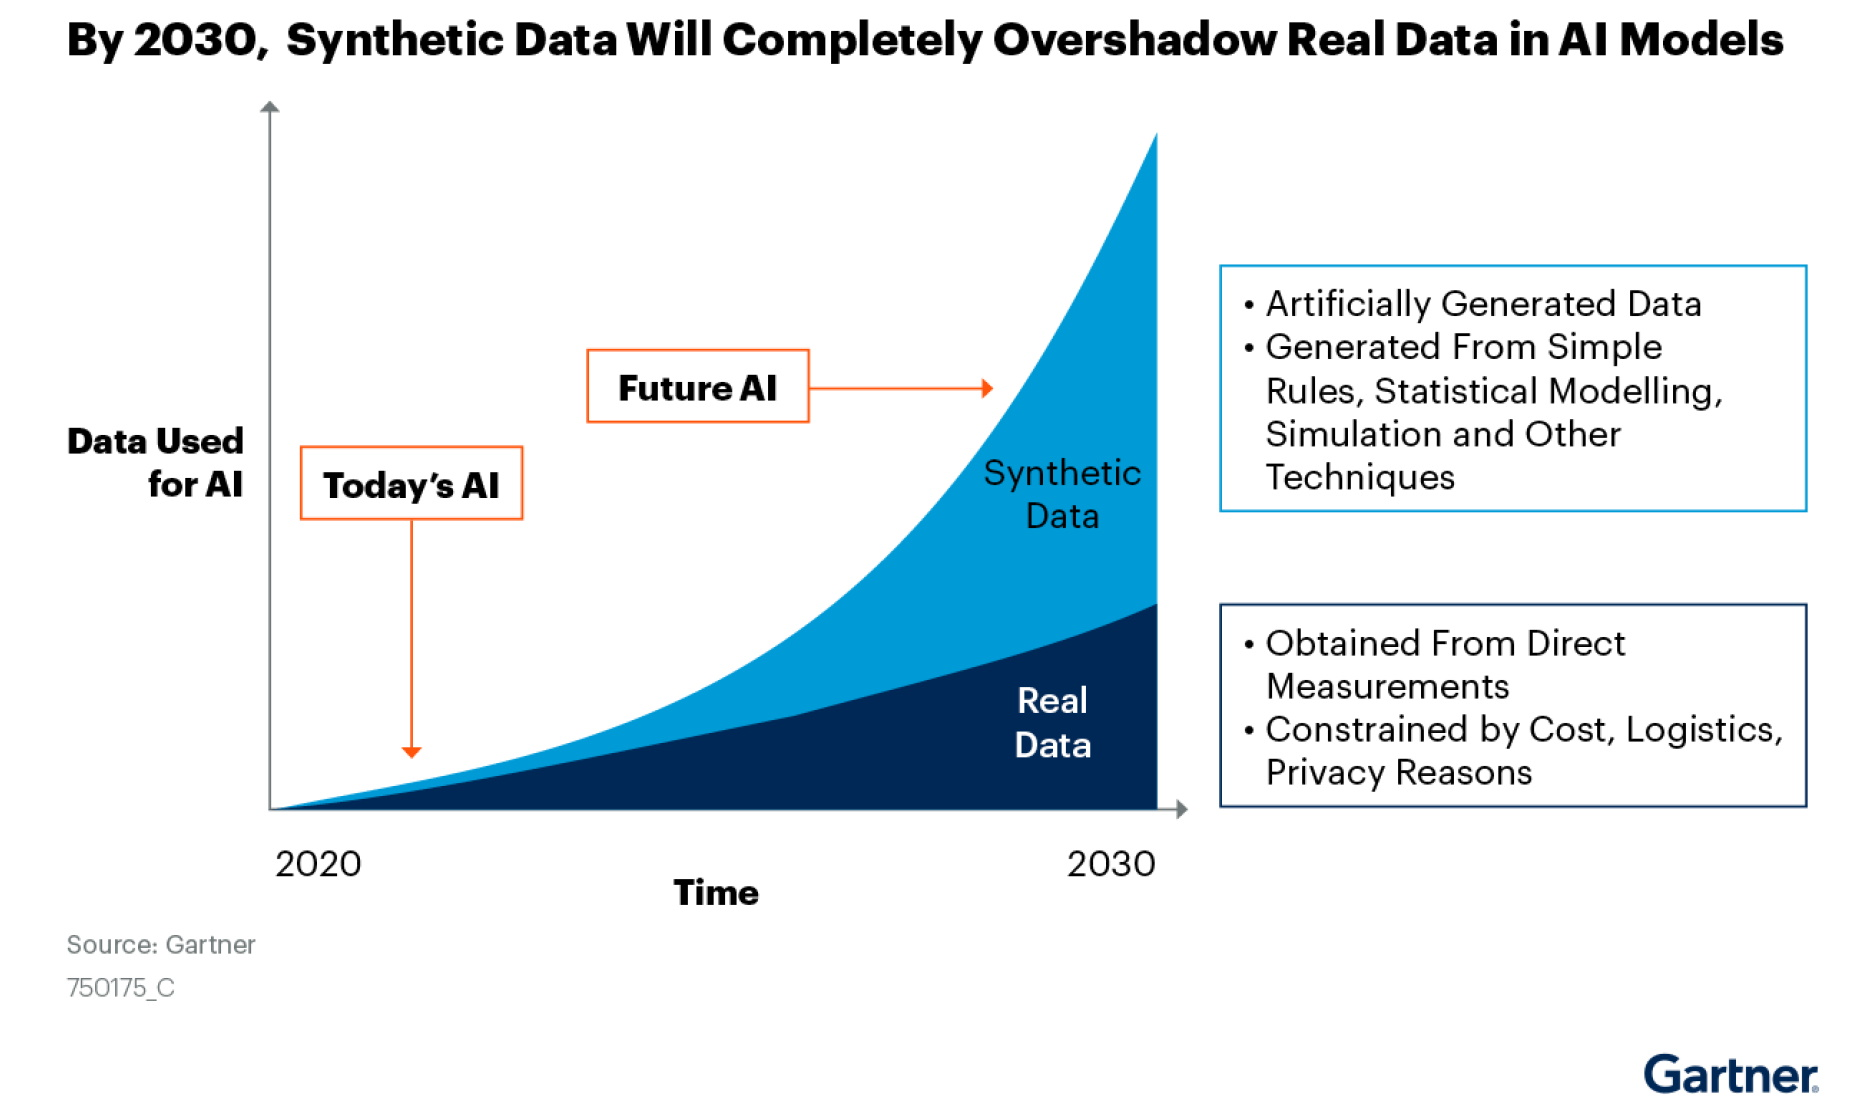
\includegraphics[width=1.0\textwidth]{/Users/apple/OVGU/Thesis/code/3dReconstruction/report/images/intro/Gartner-chart}
    \caption{A graph showing how synthetic dataset will evolve overtime ~\cite{gartnerreport}}
    \label{fig:Gartner research on synthetic dataset}
\end{figure}

Deep Learning has made leaps and bounds in solving 2D-image tasks like classification, segmentations, object detection, etc.
It has now entered the realm of Three-Dimension. An image is a 3D objects projects onto a 2D-surface.
While doing so, some data from higher dimension is being lost in lower dimension.
This inverse ability to reconstruct 3D objects from 2D images has a wide scale application in computer vision and robotics.
Tasks like human body shapes and face reconstructions ~\cite{deng2019accurate,Guo20173DFaceNetRD,9210569,richardson20163d,Richardson2017LearningDF},
3D-Scene reconstructions~\cite{Denninger20203DSR,Song2017SemanticSC,LiSilhouetteAssisted3O,Shin20193DSR}, generic object mesh reconstruction with textures are some of the advancements we had over recent years.
Here comes the challenge;3D data is not easy to collect. 3D data is not just limited but also noisy and expensive to collect.
The results of models depend on the consistency of the labelled data.
In this thesis we discuss how game engines can contribute to generating quality labeled dataset for 3D reconstruction task.

\section{Domain Adaptation vs Domain randomisation}

As mentioned earlier, the success of Convolutional Neural Networks depends highly on the training data.
As it so happens, not every task will have abundant data to train with.
One solution for this problem is using a pre-trained network of similar problem and using transfer learning.
The pre-trained network is then trained over with the limited data available for the problem at hand.
In this case the features learnt from larger dataset is fine-tuned by overwriting few layers using small annotated dataset of a different domain.
Domain adaptation is field of study in machine learning where the distribution of training data differs from testing or target distribution.
One shallow approach is as mentioned above; re-weighting the network with testing data to adapt to the problem domain ~\cite{Li2017PredictionRF}.
\todo{add more citations for domain adaptation}. "Deep domain adaptation methods
leverage deep networks to learn more transferable representations by embedding domain adaptation in the pipeline of
deep learning" ~\cite{DBLP:journals/corr/abs-1802-03601}
For this thesis, domain adaptation is relevant as synthetic dataset might not represent the real or target domain, which can lead to drop in performance.

Domain randomisation on the other hand, is improving data quality such that the target domain distribution is included in the training domain.
This is mainly used to bridge the 'reality gap' as termed in ~\cite{tobin2017domain}, between simulated environment and real images.
This is achecived by randomising the rendering of objects in the synthetic data.
The key concept here is that by rendering objects with large variance, the real-world distribution will appear to be just a variation in the dataset.
Some of the features that can be randomised in a synthetic dataset are textures, brightness, shadows, camera settings, object pose, etc. This will be further discussed in chapter \todo{mention chapter}.


\section{Volumetric representations of 3D shapes}
The universal representation of images in computer graphics is via pixels.
But unlike 2D, 3D data can be represented in various formats like voxels, mesh and point clouds. A sample of thes 3 formats is shown in ~\ref{fig:3d representation}.
Each of the representation have its own sets of advantages and disadvantages.
Voxels, which is short for Volumetric Pixels is a 3D-grid of pixels of constant size.
As indicated in ~\cite{li2016fpnn}, the main advantage of voxels is that Convolution Neural Networks can be easily applied to 3D as in 2D.
But since most of the 3D geometry is surface based, it can be wasteful and computationally expensive.
Mesh is composed of vertices, edges and faces in 3D space that indicate the formation of 3D objects.
This form of representation is far more compact at granular level depending on the resolution.
Point clouds on the other hand are collection of 3D points with (x,y,z) coordinates on the surface of the object.
The collection of points determines detailing the 3D object representation. But in both these cases CNN is not directly applicable.
In this thesis we will be dealing with voxel based models as the focus is on performance of synthetic data rather than the model or the 3d representation itself.
\todo{add an image with 3 types of represntations.}

\begin{figure}
    \centering
    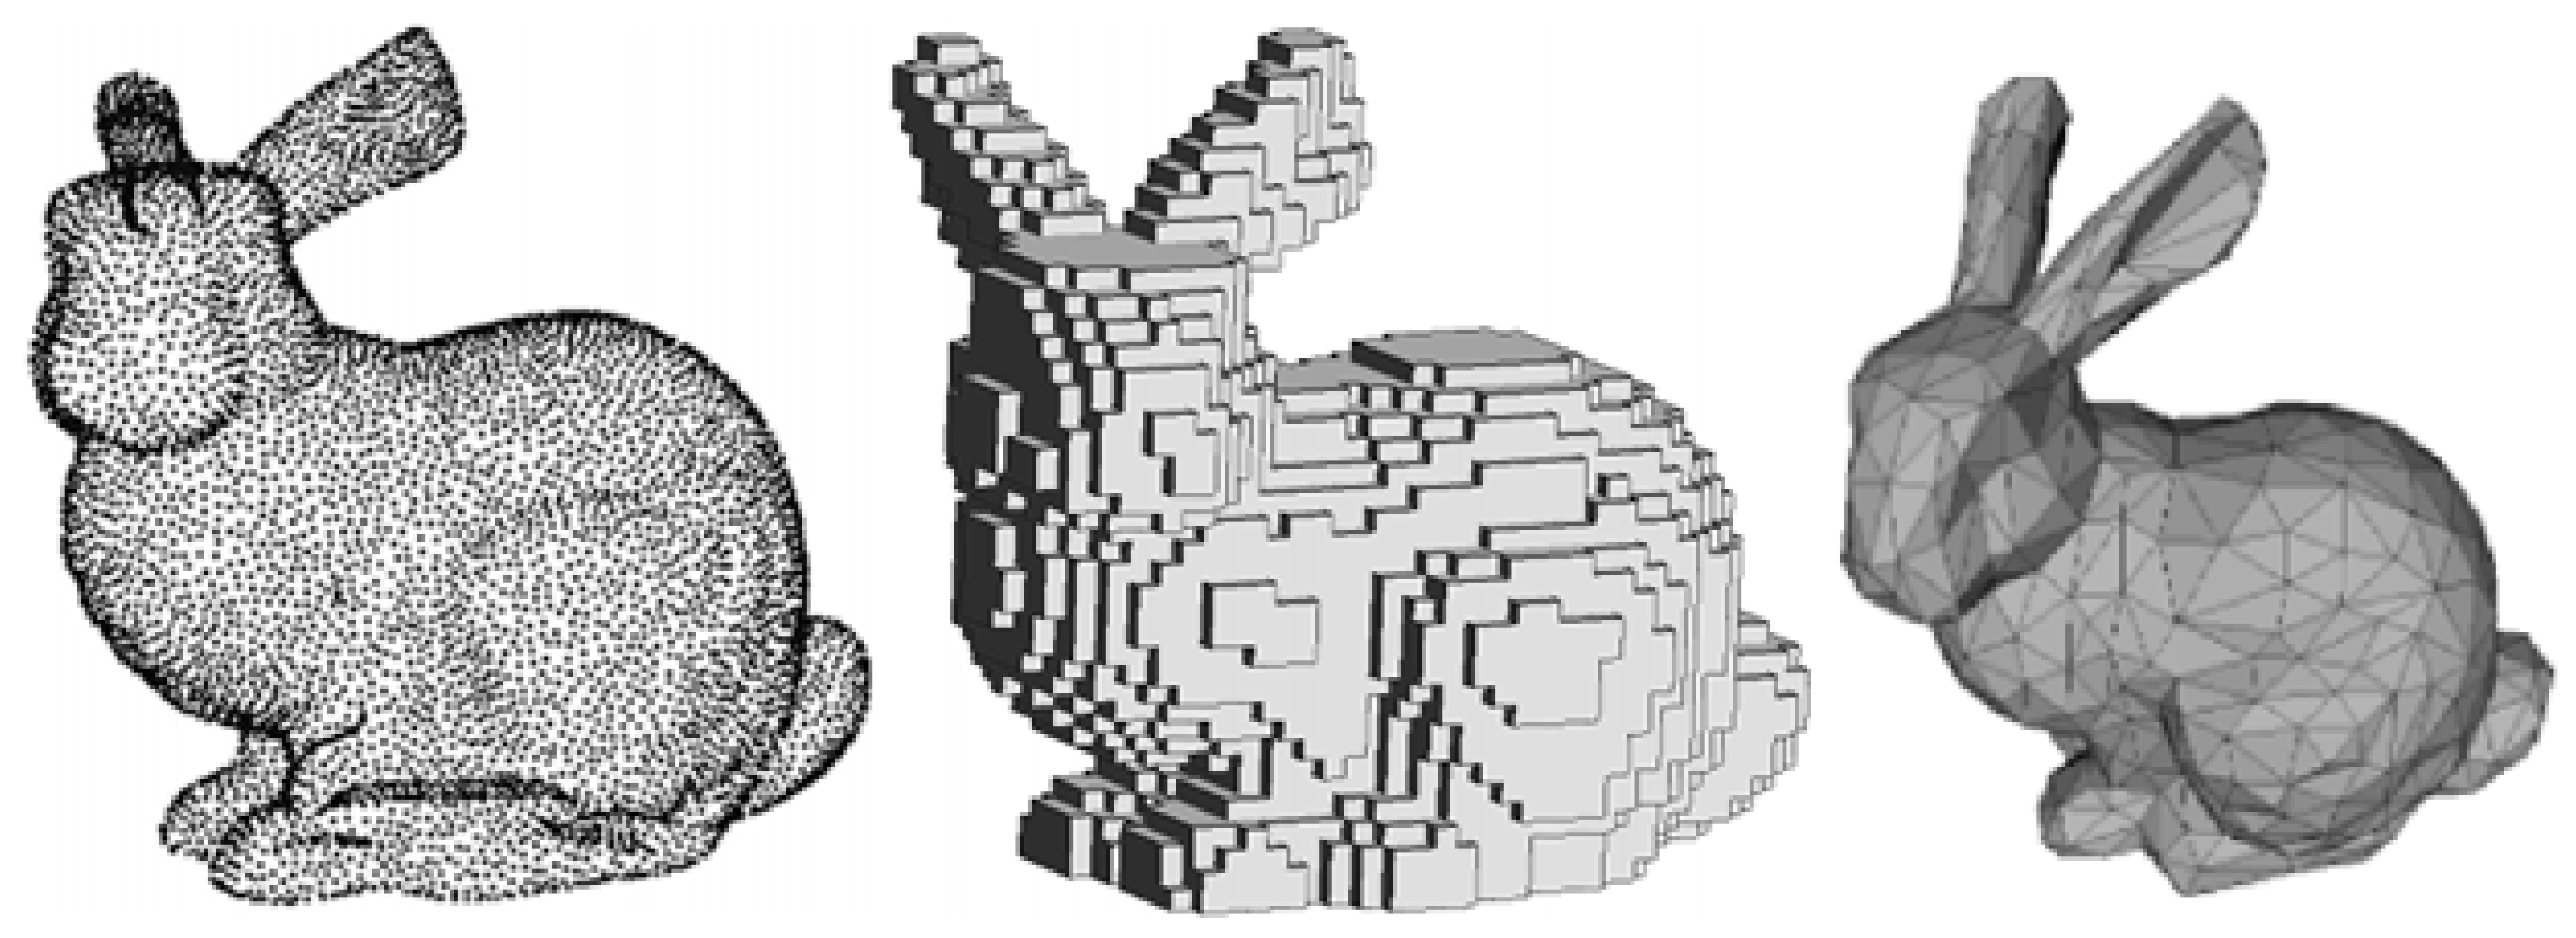
\includegraphics[width=1.0\textwidth]{/Users/apple/OVGU/Thesis/code/3dReconstruction/report/images/intro/3drepresentation}
    \caption{3D representation of Standford bunny model.(left to right) Point cloud, voel and mesh ~\cite{Hoang2019ADL}
    \label{fig:3d representation}}
\end{figure}
\section{GameEngines}

As per ~\cite{10.5555/983334}, game engine is defined as “A series of modules and interfaces that allows a
development team to focus on product gameplay content, rather than technical content”.
In layman term game engines are software used for development of games.
Unreal Engine, Unity, GameMaker, Amazon Lumeryard, CryEngine are some of the popular game engines in modern times.
Over time, the graphics in each of the game engines has improved to an extent where visually we are not able to differentiate between reality and graphics.
These use object-oriented techniques which help in modularity. Also, they are GUI-oriented and hence are user friendly and accessible even to a novice programmer.
The key component in game engines which we will be focusing on is the 'Rendering engine'. 3D Rendering is process of converting 3D data into 2D images.
Rendering can either be real-time or offline/pre-rendering. Game engines aim to make photorealism at highest level with least possible rendering time.


\section{Background and motivation}
3D reconstruction is of great significance to understand scene and to cross the 2D realm.
But the task is not trivial, considering the input is still a Two-dimensional RGB image.
It is even more challenging since obtaining new data is expensive and time-consuming.
The 3D reconstruction field has datasets like ShapeNet ~\cite{chang2015shapenet}, 3D-Front~\cite{Fu20203DFRONT3F}.
But there are no corresponding real-images to check if the model will work in real world scenarios.
Also searching for real-world examples or creating a set-up scene and then labelling the images manually can lead to human mistakes resulting in wrong labels.
A solution to this problem is automating the task of generating synthetic data which can produce pixel-perfect annotations.
This can solve human-in-the-loop problem, and while time gets saved, large quantity of data can be generated.
But quantity should not the only focus while creating the data, equal importance needs to be given to quality of the data.
Game engines have come long way from just supporting 2D to supporting games with photorealistic rendering.
Even though game engines have grown to be successful, not many tools are based on it. As 3D models available,
we can import these models into the game engine and create an ersatz environment to generate photorealistic dataset.
Further, we can check if these photorealisitc synthetic data can be used for 3D reconstruction task.

\section{Goal of this Thesis}\label{ss:goal}

The following research questions will be answered:
\begin{enumerate}
    \item Are game engines a good medium to create photorealistic synthetic dataset?
    \todo{\begin{enumerate}
        \item Experiment: Conduct a survey on real vs synthetic. Use dataset like Pix3d(real), blender proc, unity, 3d-front (synthetic)
        \item Depending on the survey, the most real dataset will be considered as baseline and other datasets will be compared to it.
    \end{enumerate} }
    \item Can Ersatz environment from a game engine like Unity replace real data for training in 3d reconstruction task?
    \todo{\begin{enumerate}
            \item Train on s2r:3dfree data, test on pix3d
        \end{enumerate}}
    \item To what extent can the performance of model Pre-trained with real dataset improved with Synthetic dataset from game engine,
            with size of synthetic dataset being 10\todo{(depends on how much data is generated)} times that of real dataset?
    \todo{\begin{enumerate}
            \item pretrained on pix3d, continue training on s2r:3dfree
            \item Mix training
    \end{enumerate}}
    \item \todo{(optional: Can the photorealism of synthetic image further be enhanced using domain adaptation/GAN techniques?)}
\end{enumerate}

\todo{Overall dataset experiments:
    \begin{enumerate}
          \item Ablation study on chairs, conduct all above mentioned experiments only on chairs as it has highest number of 3d models available
          \item Finetune chair dataset and check if dataset can be improved to get better results
          \item Scoremaps on voxel output to see if the probabilty of voxel is high in required region and to see which region is least to give possible explaination fo low IOU
\end{enumerate}}

\section{Structure of this Thesis}

The rest of this thesis is structured as follows:

\begin{itemize}
    \item \autoref{ch:related_work}, we visit some of the related work on synthetic data generation and state of the art 3d reconstruction networks.

    \item \autoref{ch:concept} deals with concepts and design choices.
x
    \item In \autoref{ch:implementation}, we discuss in detail the 3DScene tool developed using Unity game engine for creating ersatz environment.

    \item  \autoref{ch:evaluation} is dedicated to reviewing and discussing evaluation results obtained by comparison of synthetic and real dataset.

    \item Finally in \autoref{ch:conclusion}, we conclude this thesis with results of the study, highlight few limitations and discuss future improvements.

\end{itemize}